\subsubsection{Introduction}

First, we will look at the basic equation from which we will learn about the behavior of the neuron according to this model:

\begin{equation}
v(t) + \tau_m \cdot \frac{dv(t)}{dt} = E_{\text{rest}} + R_m \cdot I_{\text{input}}
\end{equation}

If we set \( R_m = 1 \) and \( E_{\text{rest}} = 0 \), the equation becomes:

\begin{equation}
v(t) + \tau_m \cdot \frac{dv(t)}{dt} = I_{\text{input}}
\end{equation}

This is a first-degree differential equation with the conditions:

\begin{equation}
v(t=0) = v_{\text{reset}}
\end{equation}

\begin{equation}
v(t=\infty) = I_0
\end{equation}

We will "guess" a solution: 

\begin{equation}
v(t) = A \cdot \exp(\alpha \cdot t) + B
\end{equation}

Our initial equation will be:

\begin{equation}
t=0 : \quad A + B = v_{\text{reset}}
\end{equation}

\begin{equation}
t=\infty : \quad B = I_0
\end{equation}

So, \( A = v_{\text{reset}} - I_0 \) and \( B = I_0 \). Substituting these values, we get:

\begin{equation}
v(t=0) + \tau_m \cdot \frac{dv(t=0)}{dt} = A + B + \tau_m \cdot A \cdot \alpha = I_0
\end{equation}

\begin{equation}
v_{\text{reset}} + \tau_m \cdot (v_{\text{reset}} - I_0) \cdot \alpha = I_0
\end{equation}

Subtracting \( v_{\text{reset}} \) from each side and dividing by \( (v_{\text{reset}} - I_0) \) to get:

\begin{equation}
\alpha = -\frac{1}{\tau_m}
\end{equation}

Overall, our solution will be:

\begin{equation} \label{eq:general_sol}
v(t) = (v_{\text{reset}} - I_0) \cdot \exp(-t/\tau_m) + I_0
\end{equation}

Now we wish to see how long it takes for our neuron to reach action potential after the most recent spike:

After \( \Delta t = t_{\text{ref}} \) the neuron will start "charging" once more (refractory period). Our initial values are as we described – we want to find a value \( t \) which will give the following:

\begin{equation}
v(t) = v_{\text{thr}}
\end{equation}

This equation has two different states – if \( I_0 < v_{\text{thr}} \) the equation has no solutions! If \( I_0 \geq v_{\text{thr}} \):

\begin{equation}
(v_{\text{reset}} - I_0) \cdot \exp(-t/\tau_m) + I_0 = v_{\text{thr}}
\end{equation}

\begin{equation}
\exp(-t/\tau_m) = \frac{v_{\text{thr}} - I_0}{v_{\text{reset}} - I_0}
\end{equation}

\begin{equation}
t = \tau_m \cdot \ln\left(\frac{v_{\text{reset}} - I_0}{v_{\text{thr}} - I_0}\right)
\end{equation}

Since our input is constant, the behavior we just got will repeat itself after each firing – in other words; the neuron will fire after:

\begin{equation}
T = t_{\text{ref}} + \tau_m \cdot \ln\left(\frac{v_{\text{reset}} - I_0}{v_{\text{thr}} - I_0}\right)
\end{equation}

So, the firing frequency is given by:

\begin{equation}
f(I_E) = \begin{cases}
    0, & \text{if } I_E < v_{\text{thresh}} \\
    \left(t_{\text{ref}} + \tau_m \cdot \ln\left(\frac{I_E - V_{\text{reset}}}{I_E - V_{\text{thresh}}}\right)\right)^{-1}, & \text{else}
\end{cases}
\end{equation}

In conclusion, we reached the frequency function:

\begin{equation}
f(I_E) = \begin{cases}
    0, & \text{if } I_E < v_{\text{thresh}} \\
    \left(t_{\text{ref}} + \tau_m \cdot \ln\left(\frac{I_E - V_{\text{reset}}}{I_E - V_{\text{thresh}}}\right)\right)^{-1}, & \text{else}
\end{cases}
\end{equation}

Now we will look at some graphs that express the influence of the \( t_{\text{refractory}} \) and \( I_E \) values on the firing frequency.

\begin{figure}[H]
    \centering
    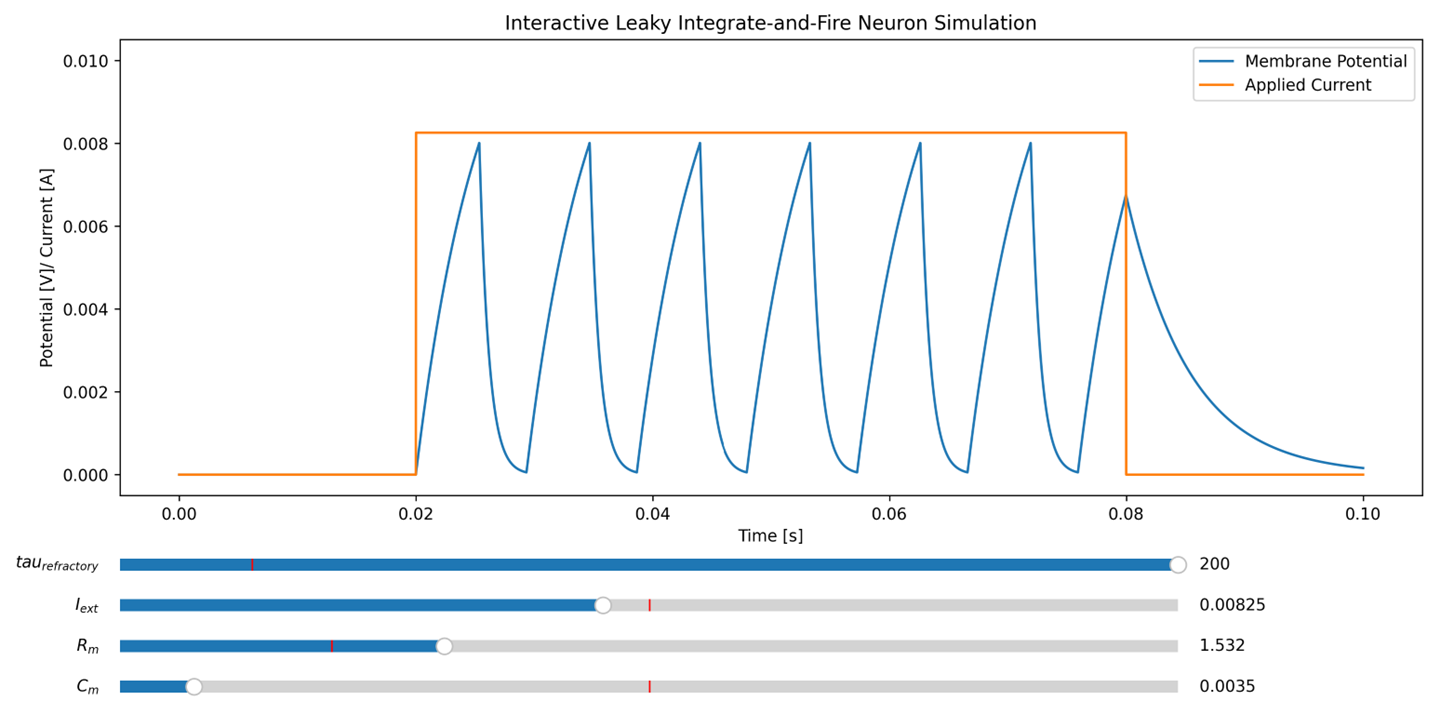
\includegraphics[width=0.6\textwidth]{scientific-background/computational-models/LIF/graphs/LIF-heaviside-high-ref.png}
    \caption{High applied current with high refractory period gives low frequency}
    \label{fig:LIF-heaviside-high-ref}
\end{figure}

\begin{figure}[H]
    \centering
    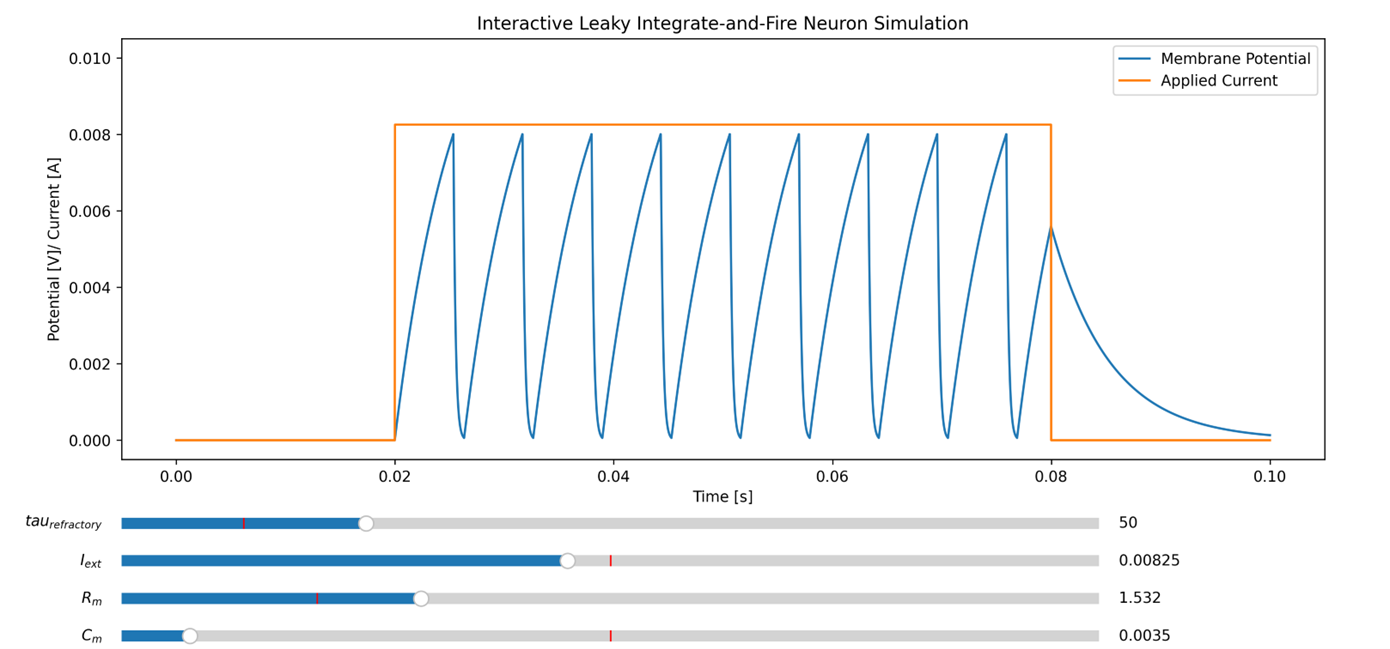
\includegraphics[width=0.6\textwidth]{scientific-background/computational-models/LIF/graphs/LIF-heaviside-low-ref.png}
    \caption{High applied current with low refractory period gives higher frequency}
    \label{fig:LIF-heaviside-low-ref}
\end{figure}

\begin{figure}[H]
    \centering
    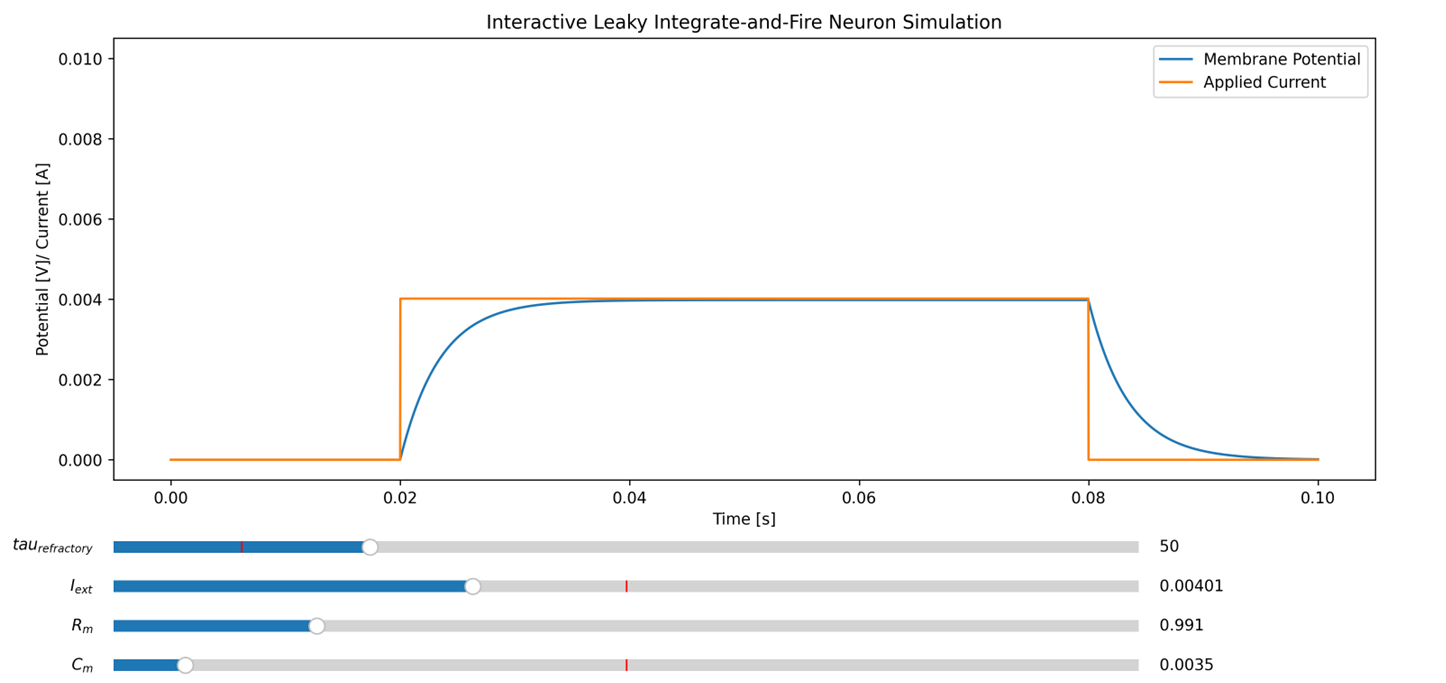
\includegraphics[width=0.6\textwidth]{scientific-background/computational-models/LIF/graphs/LIF-heaviside-low-input.png}
    \caption{Low applied current will prevent the neuron from firing}
    \label{fig:LIF-heaviside-low-input}
\end{figure}

The refractory period is a period after firing of a specific neuron during which it will ``ignore'' the input current. We can demonstrate that behavior by the following equation:
*For this example, we assume that the neuron fired at \( t=0 \).

\begin{equation}
    \forall t \in (0,\tau_{\text{ref}}), \quad I(t) = v_{\text{reset}}
\end{equation}

\begin{equation}
    v(t=0) = v_{\text{thresh}}
\end{equation}

\begin{equation}
    v(t) + \tau_m \cdot \dot{v}(t) = v_{\text{reset}}
\end{equation}

We already solved a similar equation \ref{eq:general_sol}, so the following solution will be:

\begin{equation}
    v(t) = (v_{\text{thresh}} - v_{\text{reset}}) \cdot \exp\left(-\frac{t}{\tau_m}\right) + v_{\text{reset}}
\end{equation}
These graphs portray the equation we have shown above, and as we can see, they present the behavior of the neuron model as we would have expected!
